% Options for packages loaded elsewhere
\PassOptionsToPackage{unicode}{hyperref}
\PassOptionsToPackage{hyphens}{url}
%
\documentclass[
]{article}
\usepackage{amsmath,amssymb}
\usepackage{iftex}
\ifPDFTeX
  \usepackage[T1]{fontenc}
  \usepackage[utf8]{inputenc}
  \usepackage{textcomp} % provide euro and other symbols
\else % if luatex or xetex
  \usepackage{unicode-math} % this also loads fontspec
  \defaultfontfeatures{Scale=MatchLowercase}
  \defaultfontfeatures[\rmfamily]{Ligatures=TeX,Scale=1}
\fi
\usepackage{lmodern}
\ifPDFTeX\else
  % xetex/luatex font selection
\fi
% Use upquote if available, for straight quotes in verbatim environments
\IfFileExists{upquote.sty}{\usepackage{upquote}}{}
\IfFileExists{microtype.sty}{% use microtype if available
  \usepackage[]{microtype}
  \UseMicrotypeSet[protrusion]{basicmath} % disable protrusion for tt fonts
}{}
\makeatletter
\@ifundefined{KOMAClassName}{% if non-KOMA class
  \IfFileExists{parskip.sty}{%
    \usepackage{parskip}
  }{% else
    \setlength{\parindent}{0pt}
    \setlength{\parskip}{6pt plus 2pt minus 1pt}}
}{% if KOMA class
  \KOMAoptions{parskip=half}}
\makeatother
\usepackage{xcolor}
\usepackage[margin=1in]{geometry}
\usepackage{graphicx}
\makeatletter
\def\maxwidth{\ifdim\Gin@nat@width>\linewidth\linewidth\else\Gin@nat@width\fi}
\def\maxheight{\ifdim\Gin@nat@height>\textheight\textheight\else\Gin@nat@height\fi}
\makeatother
% Scale images if necessary, so that they will not overflow the page
% margins by default, and it is still possible to overwrite the defaults
% using explicit options in \includegraphics[width, height, ...]{}
\setkeys{Gin}{width=\maxwidth,height=\maxheight,keepaspectratio}
% Set default figure placement to htbp
\makeatletter
\def\fps@figure{htbp}
\makeatother
\setlength{\emergencystretch}{3em} % prevent overfull lines
\providecommand{\tightlist}{%
  \setlength{\itemsep}{0pt}\setlength{\parskip}{0pt}}
\setcounter{secnumdepth}{-\maxdimen} % remove section numbering
\usepackage{booktabs}
\usepackage{longtable}
\usepackage{array}
\usepackage{multirow}
\usepackage{wrapfig}
\usepackage{float}
\usepackage{colortbl}
\usepackage{pdflscape}
\usepackage{tabu}
\usepackage{threeparttable}
\usepackage{threeparttablex}
\usepackage[normalem]{ulem}
\usepackage{makecell}
\usepackage{xcolor}
\ifLuaTeX
  \usepackage{selnolig}  % disable illegal ligatures
\fi
\IfFileExists{bookmark.sty}{\usepackage{bookmark}}{\usepackage{hyperref}}
\IfFileExists{xurl.sty}{\usepackage{xurl}}{} % add URL line breaks if available
\urlstyle{same}
\hypersetup{
  pdftitle={HW3},
  pdfauthor={Denys Osmak},
  hidelinks,
  pdfcreator={LaTeX via pandoc}}

\title{HW3}
\author{Denys Osmak}
\date{2024-02-03}

\begin{document}
\maketitle

\hypertarget{github}{%
\subsection{Github:}\label{github}}

\hypertarget{problem-1}{%
\section{Problem 1:}\label{problem-1}}

\hypertarget{a-what-creatinine-clearance-rate-should-we-expect-for-a-55-year-old-explain-briefly-one-or-two-sentences-equations-how-you-determined-this.}{%
\subsection{A) What creatinine clearance rate should we expect for a
55-year-old? Explain briefly (one or two sentences+ equations) how you
determined
this.}\label{a-what-creatinine-clearance-rate-should-we-expect-for-a-55-year-old-explain-briefly-one-or-two-sentences-equations-how-you-determined-this.}}

Using the formula \[ y = 172.283 - 1.085x \] where y represents the
creatine rate and x represents the age. We can plug in 55 for the x and
determine that a 55 year old's kidney should produce 112.6 mL of
creatine per minute.

\hypertarget{b-how-does-creatinine-clearance-rate-change-with-age-this-should-be-a-single-number-whose-units-are-mlminute-per-year.-explain-briefly-one-or-two-sentences-how-you-determined-this}{%
\subsection{B) How does creatinine clearance rate change with age? (This
should be a single number whose units are ml/minute per year.) Explain
briefly (one or two sentences) how you determined
this}\label{b-how-does-creatinine-clearance-rate-change-with-age-this-should-be-a-single-number-whose-units-are-mlminute-per-year.-explain-briefly-one-or-two-sentences-how-you-determined-this}}

Using the formula \[ y = 172.283 - 1.085x \] where y represents the
creatine rate and x represents the age. We can see that the creating
clearance rate decreases by 1.085 mL/min per year.

\hypertarget{c-whose-creatinine-clearance-rate-is-healthier-higher-for-their-age-a-40-year-old-with-a-rate-of-135-or-a-60-year-old-with-a-rate-of-112-explain-briefly-a-few-sentences-equations-how-you-determined-this.}{%
\subsection{C) Whose creatinine clearance rate is healthier (higher) for
their age: a 40-year-old with a rate of 135, or a 60-year-old with a
rate of 112? Explain briefly (a few sentences + equations) how you
determined
this.}\label{c-whose-creatinine-clearance-rate-is-healthier-higher-for-their-age-a-40-year-old-with-a-rate-of-135-or-a-60-year-old-with-a-rate-of-112-explain-briefly-a-few-sentences-equations-how-you-determined-this.}}

By pluging in our formula, we predict that the 40 year old will have a
creatine clearance rate of 128.883, while his actual rate is 135,
meaning that his rate is 6.117 above normal. While we can predict that a
60 year old will have a clearance rate of 107.183, while his actual rate
is 112, meaning that his rate is 4.817 above normal. Since the 40 year
old's clearance rate residual is higher then the 60 year old's, it means
he is healthier for this age.

\hypertarget{problem-2}{%
\section{Problem 2}\label{problem-2}}

\hypertarget{what-is-beta-in-financial-world}{%
\subsection{What is ``beta'' in financial
world?}\label{what-is-beta-in-financial-world}}

A beta value in the financial world means how closely related the stock
is to the overall stock market performance, or how much of the risk
comes from the market volatility (also called systematic risk). The
larger the beta value the larger the systematic risk is. The beta number
ranges from 0 - 1. 1 meaning for every point the market goes up or down,
so does this individual stock. While a value of 0 means that the
individual stock does not respond to the stock market at all, no matter
if it goes up or down. There are also a few other occasions where the
beta value is over 1 and a negative value. If the beta is over 1, that
means for every 1 point the market goes up the individual stock
outproduces the market. While a negative beta value means an inverse
correlation to market, meaning if the market goes down this individual
stock goes up.

\hypertarget{table}{%
\subsection{Table}\label{table}}

\hypertarget{systematic-risk-of-the-stocks}{%
\subsection{Systematic risk of the
stocks}\label{systematic-risk-of-the-stocks}}

\hypertarget{problem-3}{%
\section{Problem 3}\label{problem-3}}

\hypertarget{an-estimated-growth-rate-and-doubling-time-for-italy.}{%
\subsection{1. An estimated growth rate and doubling time for
Italy.}\label{an-estimated-growth-rate-and-doubling-time-for-italy.}}

Our estimated growth rate for Ovid death rate in Italy is 18.321\%,
meaning that by using the rule of 70 \[ 70/18.321 = 3.82\], meaning that
the Covid death toll will double every 4 days during the begging of this
epidemic.

\hypertarget{an-estimated-growth-rate-and-doubling-time-for-spain.}{%
\subsection{2. An estimated growth rate and doubling time for
Spain.}\label{an-estimated-growth-rate-and-doubling-time-for-spain.}}

Our estimated growth rate for Ovid death rate in Italy is 27.624\%,
meaning that by using the rule of 70 \[ 70/27.624 = 2.52\], meaning that
the Covid death toll will double every 3 days during the begging of this
epidemic.

\hypertarget{a-line-graph-showing-reported-daily-deaths-over-time}{%
\subsection{3. A line graph showing reported daily deaths over
time}\label{a-line-graph-showing-reported-daily-deaths-over-time}}

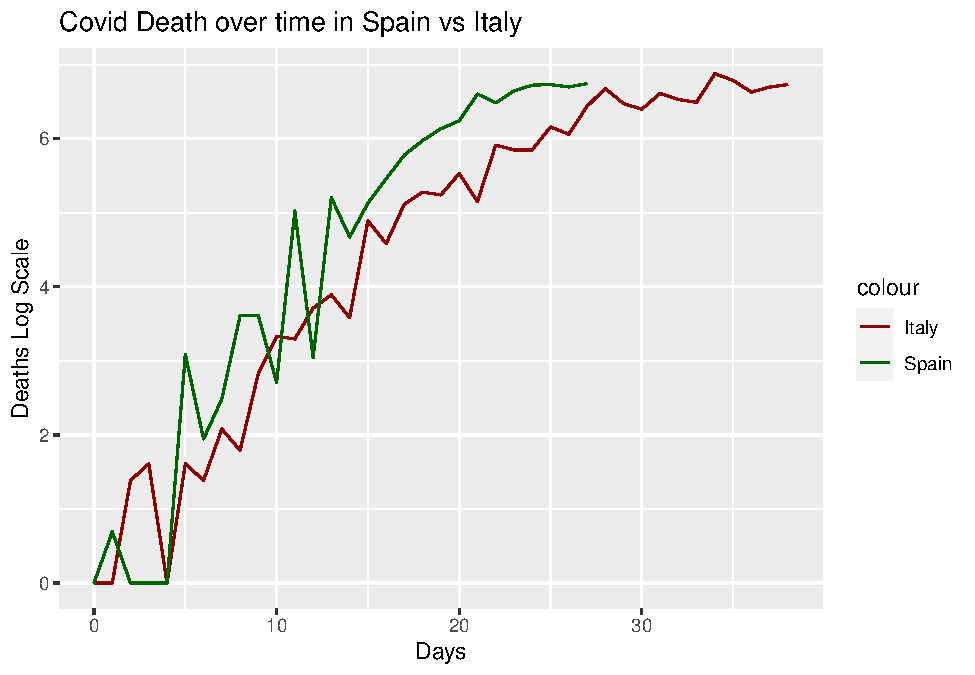
\includegraphics{HW3_files/figure-latex/unnamed-chunk-8-1.pdf}

\hypertarget{problem-4}{%
\section{Problem 4}\label{problem-4}}

In light of the data, what is the estimated price elasticity of demand
for milk? Briefly describe what you did no more than a few sentences,
together with your estimate.

For every 1\% the price increases the sales of milk drop by 1.619\%.
Because the demand for the good goes down with the price increase this
makes milk an elastic good.

\end{document}
